\documentclass[12pt,twoside]{article}
\usepackage{amsmath, amssymb}
\usepackage{amsmath}
\usepackage[active]{srcltx}
\usepackage{amssymb}
\usepackage{amscd}
\usepackage{makeidx}
\usepackage{amsthm}
\usepackage{algpseudocode}
\usepackage{algorithm}
\usepackage[spanish]{babel}
\usepackage[usenames]{color}

\usepackage{fancyhdr}
\usepackage{graphics}
\usepackage{listings}
%----------------------------------------------------------------------------------------------
\usepackage{amsmath, amssymb}
\usepackage{amsmath}
\usepackage[active]{srcltx}
\usepackage{amssymb}
\usepackage{amscd}
\usepackage{makeidx}
\usepackage[dvips]{graphicx}
\usepackage{booktabs,array,arydshln}
\usepackage[export]{adjustbox}
\usepackage{caption}
\usepackage{subcaption}
\usepackage{siunitx}
\usepackage{etoolbox}
\usepackage[backend=biber]{biblatex}
\addbibresource{bibliografia.bib}

\renewcommand{\baselinestretch}{1}
\setcounter{page}{1}
\setlength{\textheight}{21.6cm}
\setlength{\textwidth}{14cm}
\setlength{\oddsidemargin}{1cm}
\setlength{\evensidemargin}{1cm}
\pagestyle{myheadings}
\thispagestyle{empty}
\markboth{\small{Pr\'actica 3. Catonga Tecla Daniel Isaí 1, Olguin Castillo Victor Manuel 2.}}{\small{.}}
\date{}
\begin{document}



\begin{figure}[h]
\vspace{-3cm} \hspace{-2cm} \setlength{\unitlength}{1mm}
\begin{picture}(15,25)(-10,0)

\includegraphics[width=16cm,height=3cm]{titulo.jpg}
\end{picture}
\end{figure}


\vspace{0cm}

\centerline{\bf Ingeniería en Inteligencia Artificial, An\'alisis y Diseño de Algoritmos}

\centerline{\bf Sem: 2024-1, 3BV1, Pr\'actica 3, 18 de octubre de 2023}

\centerline{}

%\centerline{}


\begin{center}
\Large{\textsc{Pr\'actica 3: Funciones Recursivas vs Iterativas.}}
\end{center}
\centerline{}
\centerline{\bf {Catonga Tecla Daniel Isaí 1, Olguin Castillo Victor Manuel 2.}}
\centerline{}
\centerline{$daniel9513importantes@gmail.com_1, manuelevansipn@gmail.com_2$}



\newtheorem{Theorem}{\quad Theorem}[section]

\newtheorem{Definition}[Theorem]{\quad Definition}

\newtheorem{Corollary}[Theorem]{\quad Corollary}

\newtheorem{Lemma}[Theorem]{\quad Lemma}

\newtheorem{Example}[Theorem]{\quad Example}

\bigskip

\textbf{Resumen:}\\





{\bf Palabras Clave:} Algoritmo, Big O, C++, Recursividad

%----------------------------------------------- INTRODUCCIÓN
\newpage
\section{Introducci\'on}

Un algoritmo es un conjunto ordenado y finito de operaciones que permite hallar la solución de un problema \cite{algoritmo}. 
Los algoritmos son de suma importancia, estos ayudan a la resolución de problemas muy grandes o complejos como problemas matemáticos y científicos, por lo tanto, los 
algoritmos son fundamentales en varias áreas de las ciencias o ingeniería.

\par 
En programación, las operaciones pueden ser manejadas por recursividad o iteraciones. 
Recursividad es una función que se llama a sí misma, directa o indirectamente. Una de las estructuras fundamentales de programación son los bucles, 
las cuales forman parte de las estructuras de la mayoría de los lenguajes, los bucles sirven para los algoritmos iterativos. \cite{recuranditet}

\medskip

El análisis de algoritmos es otro parte fundamental por lo que los algoritmos tienen que ser los más eficientes posibles en complejidad temporal y complejidad espacial. 
En cuestión de complejidad temporal algunos algoritmos 
pueden requerir años en resolver un solo problema, por lo que, no es suficiente para la práctica.
, y se opta por otros algoritmos que resuelvan el problema que presenten de una forma más eficaz. Por otra parte, una maquina no cuenta con recursos infinitos de memoria o espacio de almacenamiento, por lo que, existen 
algoritmos que ocupan mucho espacio de memoria y esto puede ocasionar problemas para equipos que no cuentan con el espacio suficiente, entonces se tiene que analizar también lo que es la complejidad espacial para tratar de ocupar 
la menor cantidad de memoria posible. Ambas complejidades son importantes, pero es más importante la complejidad 
temporal ya que las empresas pueden comprar más memorias de almacenamiento, pero no pueden comprar tiempo, por lo que algunas empresas optan sacrificar complejidad espacial por una complejidad temporal más eficiente.

\medskip

Algunos algoritmos iterativos se pueden hacer de forma recursiva y viceversa, lo importante es conocer cuál es de menor complejidad de tiempo, por lo que, es importante conocer la complejidad de cada algoritmo en 
la forma recursiva o iterativa y compararlas para saber que algoritmo implementar en un caso práctico. 

\newpage


\newpage
\section{Conceptos Basicos}

\begin{itemize}
\item \textbf{Algoritmo}. Un algoritmo es una secuencia de pasos lógicos que son precisos, ordenados y finitos que se ocupan para resolver un problema deseado \cite{concep1}.

\item \textbf{Análisis de  algoritmos}
Es un proceso de evaluación donde conoceremos el rendimiento y la eficiencia de un algoritmo. Se evaluará el consumo de tiempo y de recursos computacionales que requiere el algoritmo para ser ejecutado con diversos datos de entrada, y esto determinará su complejidad \cite{concep1}.

\item \textbf{Cota superior asintótica}. Es una función que delimita por la parte superior a otra función a medida que la entrada de la función delimitada crece.

\item \textbf{Cota inferior asintótica}. Es una función que delimita por la parte inferior a otra función a medida que la entrada de la función delimitada crece.

\item \textbf{Notacion O}. Esta notación se ocupa para describir la complejidad de un algoritmo definiendo una cota superior asintótica en el peor caso de ejecución de un algoritmo \cite{concep1}.
\\
\[O(g(n)) = \{ f : \mathbb{N} \rightarrow \mathbb{R}^+ \ | \ \exists \ c \text{ constante positiva y } n_0 \notin \mathbb{N} :\] 
\[f(n) \leq cg(n), \ \forall \ n \geq n_0 \}\]

\item \textbf{Notacion Tetha "$\Theta$"} Esta notación se ocupa para describir la complejidad de un algoritmo definiendo una cota superior y una cota inferior, esto nos da una idea más precisa del comportamiento y complejidad del mismo \cite{concep1}.
\\
\[\Theta(g(n) = \{f : \mathbb{N} \rightarrow \mathbb{R}^+ \,|\, \exists \, c_1, c_2 \text{ constantes positivas}, n_0 \,: \]
\[0 < c_1g(n) \leq f(n) \leq c_2g(n), \forall \, n \geq n_0\}\]

\item \textbf{Notacion Omega "$\Omega$"}  Esta notación se ocupa para describir la complejidad de un algoritmo definiendo una cota inferior asintótica en el peor caso de ejecución de un algoritmo \cite{concep1}.
\\
\[\Omega(g(n)) = \{f : \mathbb{N} \rightarrow \mathbb{R}^+ \,|\, \exists \, c \text{ constante positiva y } n_0 \,:\]
\[0 < cg(n) \leq f(n), \forall \, n \geq n_0\}\]


\item \textbf{Analisis a posteriori}. Es una evaluación que se realiza de forma empírica, donde los resultados se obtienen con la ejecución del algoritmo y la medición del tiempo y recursos computacionales que requiere \cite{concep1}.

\item \textbf{Analisis a priori}. Es una evaluacion que se realiza de forma teorica, donde los resultados se pueden obtener con el conteo de operaciones y/o analisis matematico que en base a sus formulas se obtiene su complegidad algoritmica \cite{concep1}.

\item \textbf{Funciones recursivas}. En la programacion las funciones recursivas son aquellas que durante su proceso se invocan asi mismas.

\begin{centering}
\begin{verbatim}
                    Suma_Recursiva(n):
                    If n == 1
                        return 1 
                    Else
                        return n + sumaRecursiva(n - 1)
\end{verbatim}
\end{centering}

\item \textbf{Funciones iterativas}. En la programacion las funciones iterativas son aquellas se ejecuta en un ciclo n numero de veces y existe una condicion de validacion en cada iteracion que controla si se itera una ves mas o finaliza en ciclo

\begin{centering}
\begin{verbatim}
                    Suma_iterativa(n):
                    resultado = 0
                    for i = 0 to n do:
                        resultado += i
                    return resultado
\end{verbatim}
\end{centering} 

\item \textbf{Pseudocódigo de Búsqueda iterativo}.
El algoritmo de búsqueda, retorna el índice del valor que se busca dividiendo el arreglo en 3 partes por cada operación
que se realiza hasta encontrar el valor o en caso contrario retorna -1 si no existe el valor en el arreglo.
\begin{center}
\begin{verbatim}
            BusquedaIterativa(Arr[1,2,...,n],valor):
            low = 0
            high = longitud del vector - 1
            i entero 
            j entro
            while low <= high do:
              i = low + (high-low)/3
              j = low + 2*(high-low)/3
              if Arr[j]<valor do:
                low = j+1
              else if Arr[i]>valor do:
                high = i-1
              else if Arr[i]<valor and Arr[j]>valor do:
                low = i+1
                high = j-1
              else if Arr[i] == valor do:
                return i
              else if Arr[j] == valor do:
                return j
            return -1
\end{verbatim}
\end{center}
\item \textbf{Pseudocódigo de Búsqueda recursiva}.
El algoritmo de búsqueda recursivo se llama así msimo varias veces, retorna el índice del valor que se busca dividiendo el arreglo en 3 partes por cada operación
que se realiza hasta encontrar el valor o en caso contrario retorna -1 si no existe el valor en el arreglo.
\begin{center}
\begin{verbatim}
      BusquedaRecursiva(Arr[1,2,...,n],low,high,valor):
      if low <= high do:
        i = low + (high-low)/3
        j = low + 2*(high-low)/3
         
        if Arr[j]<valor do:
          return BusquedaRecursiva(Arr,j+1,high,valor)
        else if Arr[i]>valor do:
          return BusquedaRecursiva(Arr,low,i-1,valor)
        else if Arr[i]<valor and Arr[j]>valor do:
          return BusquedaRecursiva(Arr,j+1,i-1,valor)
        else if Arr[i] == valor do:
          return i
        else if Arr[j] == valor do:
          retur
      else:
        return -1
\end{verbatim}
\end{center}

\end{itemize}
\newpage
%------------------------------------------- EXPERIMENTACIÓN Y RESULTADOS
\section{Experimentación y Resultados}
\textbf{2. Algoritmo de Búsqueda}
\par

%---------------------------------------------- Algoritmo Iterativo Busqueda Ternaria
\textbf{Análisis a priori de algoritmo de Búsqueda Iterativo.} 
El análisis a priori del algoritmo de búsqueda iterativa se basa con el pseudocódigo del algoritmo que se muestra a continuación, titulado "BusquedaIterativa". 

\medskip
\begin{center}
  Pseudocódigo de Busqueda iterativa
  \begin{verbatim}
            BusquedaIterativa(Arr[1,2,...,n],valor):
            01.  low = 0
            02.  high = longitud del vector - 1
            03.  i entero 
            04.  j entro
            05.  while low <= high do:
            06.   i = low + (high-low)/3
            07.   j = low + 2*(high-low)/3
            08.   if Arr[j]<valor do:
            09.     low = j+1
            10.   else if Arr[i]>valor do:
            11.    high = i-1
            12.   else if Arr[i]<valor and Arr[j]>valor do:
            13.    low = i+1
            14.    high = j-1
            15.   else if Arr[i] == valor do:
            16.    return i
            17.   else if Arr[j] == valor do:
            18.    return j
            19.  return -1
  \end{verbatim}
  \end{center}
\newpage
El algoritmo posee una ecuación de recurrencia, la cual se expresa como $T(n) = T(\frac{n}{3})+C$. Esta ecuación se deriva del cálculo de la complejidad por bloques de la figura n.
  \begin{figure}[h]
    \begin{center}
      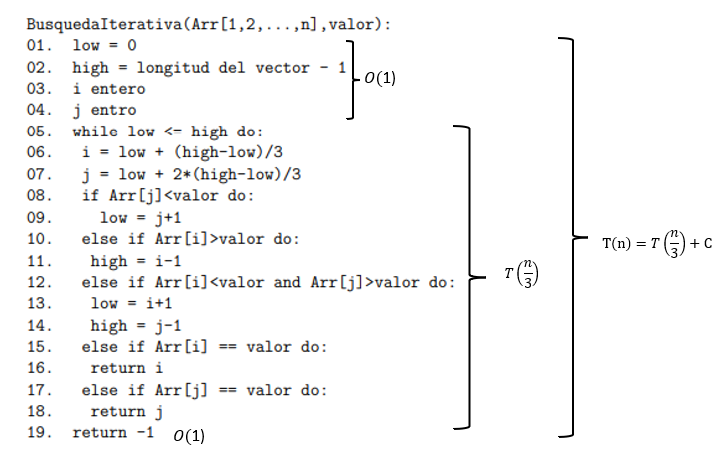
\includegraphics[width=0.85\linewidth]{images/apriori1.png}
      \\
      Figura n. Ecuación de Recurrencia.
    \end{center}
  \end{figure}

  Por lo tanto la solución de la ecuación de recurrencia se obtiene por sustitución hacía atrás. 
  
  Solución:


  $T(n)=T(\frac{n}{3})+C$

  Sea $n=3^k\ (k=log_3 n)$
  
  $\Rightarrow T(3^k)=T(3^{k-1})+C$
  \par
Resolviendo mediante sustitución hacía atrás se tiene:

  $\ \ \ \ \ \ \ \ \ \ \ \ =[T(3^{k-2})+C]+C$

  $\ \ \ \ \ \ \ \ \ \ \ \ =T(3^{k-2})+2C$

  $\ \ \ \ \ \ \ \ \ \ \ \ =[T(3^{k-3})+C]+2C$

  $\ \ \ \ \ \ \ \ \ \ \ \ =(3^{k-3})+3C$

  $\ \ \ \ \ \ \ \ \ \ \ \ \ \vdots$

  $\ \ \ \ \ \ \ \ \ \ \ \ =T(3^{k-i})+iC$

  $\ \ \ \ \ \ \ \ \ \ \ \ \ \vdots \ \ \ \ \ \ \ \  \ \ \ \ k-i=0\ \Rightarrow \ k=i$
  

  $\ \ \ \ \ \ \ \ \ \ \ \ =T(1)+kC$

  $\ \ \ \ \ \ \ \ \ \ \ \ =C+kC$

  $\ \ \ \ \ \ \ \ \ \ \ \ =C+log_3(n)C$

\par

  El algoritmo tiene complejidad:
\begin{center}
  $\therefore T(n)\in O(log_3n)$ 
\end{center}
  

\newpage
\textbf{Análisis a posteriori del algoritmo de búsqueda iterativa.}
El algoritmo en ejecución se muestra en la figura 5, y el número de pasos se muestra en la tabla 6. Los datos muestran un aumento logarítmico base 3 en la complejidad a medida que $n$ crece. Para la tabla de datos, considera que, para el peor caso, el valor que se busca no se encuentra en el vector o arreglo.
\par

\begin{minipage}{.45\linewidth}
  \centering
  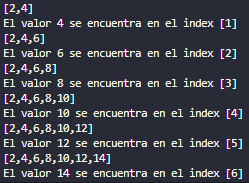
\includegraphics[width=1\linewidth]{images/busquedaiterativa.png}
  \\
  Figura 5. Ejecución de algoritmo de búsqueda iterativa.
\end{minipage}\hfill
\begin{minipage}{.45\linewidth}
  \centering
  \begin{tabular}{|c|c|}
    \hline
    \textbf{Valor de $n$} & \textbf{\# de pasos} \\
    \hline
    2  & 14 \\
    3  & 14 \\
    4  & 14 \\
    5  & 18 \\
    6  & 18 \\
    7  & 18 \\
    8  & 18 \\
    9  & 18 \\
    10 & 18 \\
    11 & 18 \\
    12 & 18 \\
    13 & 18 \\
    14 & 22 \\
    15 & 22 \\
    \vdots & \vdots\\
    \hline
  \end{tabular}
  \\
  Tabla 6. Datos de algoritmo de búsqueda iterativa.
\end{minipage}

\medskip

Los datos de ejecución del algoritmo de búsqueda iterativa se muestran en la figura 6. El algoritmo muestra un
crecimiento logaritmico base 3.

\medskip

\begin{minipage}{\linewidth}
  \centering
  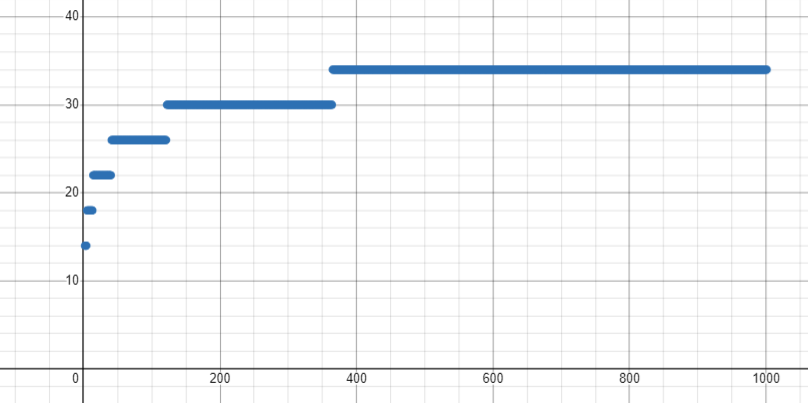
\includegraphics[width=0.7\linewidth]{images/busquedaiterativaworscase.png}
  \\
  Figura 6. Gráfica del comportamiento del algoritmo de búsqueda iterativa.
\end{minipage}
\newpage

En la figura 7 se muestra la función tal que $g(n)=7.5log_3(n)$ acota por arriba al algoritmo. El ajuste asíntotico es para cuando $n_0\geq 120$. En la figura 8 se muestra que $f(n)$ esta delimitado por $g(n)$ cuando $n\geq n_0$.
\medskip
\begin{figure}[h]
  \begin{center}
    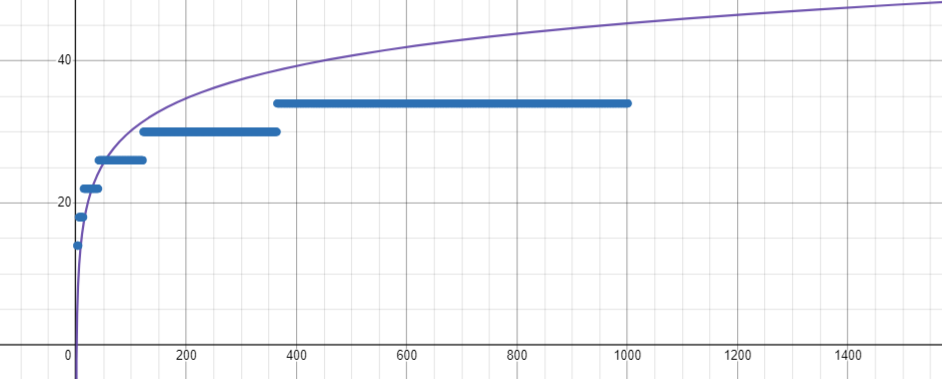
\includegraphics[width=0.7\linewidth]{images/busquedaiterativaworscasegn.png}
    \\
    Figura 7. Gráfica con acotación para $f(n)$.
  \end{center}
\end{figure}
\begin{figure}[h]
  \begin{center}
    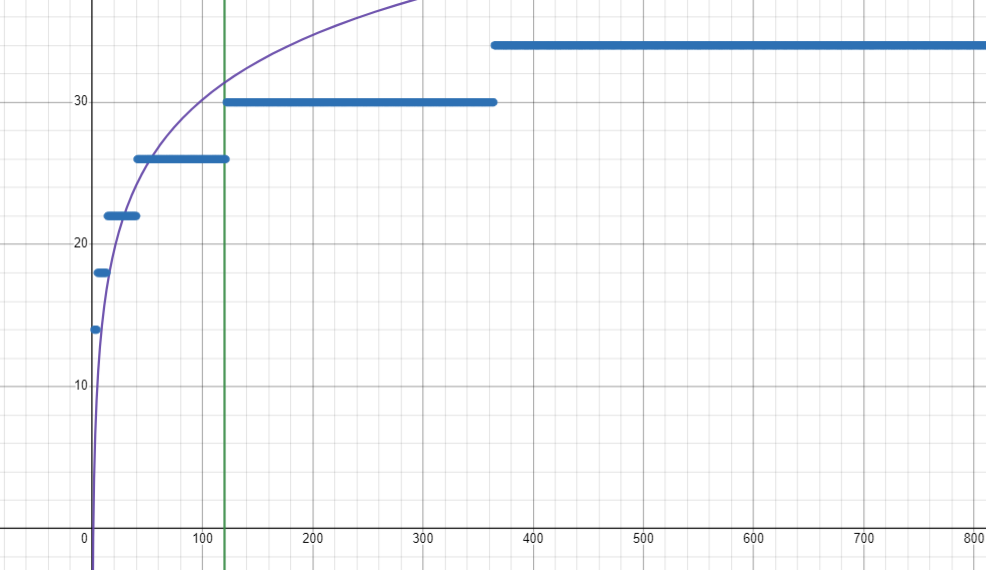
\includegraphics[width=0.7\linewidth]{images/busquedaiterativaworscasegnacotado.png}
    \\
    Figura 8. Gráfica para valor $n_0$.
  \end{center}
\end{figure}

\medskip
Por lo tanto, en el análisis a posteriori se muestra que el algoritmo es:
\begin{center}
  $\therefore T(n)\in O(log_3n)$
\end{center}

\newpage

%------------------------------- ALGORITMO DE BÚSQUEDA RECURSIVA.

\textbf{Análisis a priori de algoritmo de Búsqueda Recursivo.} 
El análisis a priori del algoritmo de búsqueda recursivo se basa con el pseudocódigo del algoritmo que se muestra a continuación, titulado "BusquedaRecursiva". 
\par
\begin{center}
  \begin{verbatim}
        BusquedaRecursiva(Arr[1,2,...,n],low,high,valor):
        01.  if low <= high do:
        02.  i = low + (high-low)/3
        03.  j = low + 2*(high-low)/3
        04.  if Arr[j]<valor do:
        05.    return BusquedaRecursiva(Arr,j+1,high,valor)
        06.  else if Arr[i]>valor do:
        07.    return BusquedaRecursiva(Arr,low,i-1,valor)
        08.  else if Arr[i]<valor and Arr[j]>valor do:
        09.    return BusquedaRecursiva(Arr,j+1,i-1,valor)
        10.  else if Arr[i] == valor do:
        11.    return i
        12.  else if Arr[j] == valor do:
        13.    return j
        14.  return -1
  \end{verbatim}
  \end{center}
\par

El algoritmo posee una ecuación de recurrencia, la cual se expresa como $T(n)=T(\frac{n}{3}+C)$. Esta ecuación se deriva a  partir del cálculo de la complejidad por bloques de la figura n.

\begin{figure}[h]
  \begin{center}
    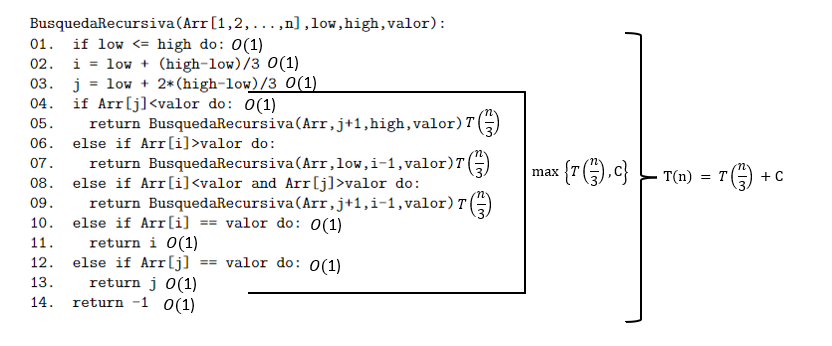
\includegraphics[width=0.85\linewidth]{images/apriori2.png}
    \\
    Figura n. Ecuación de Recurrencia.
  \end{center}
\end{figure}

\newpage
Por lo tanto, la solución de la ecuación de recurrencia se obtiene por sustitución hacía atrás. 
  
Solución:


  $T(n)=T(\frac{n}{3})+C$

  Sea $n=3^k\ (k=log_3 n)$
  
  $\Rightarrow T(3^k)=T(3^{k-1})+C$
  \par
  Resolviendo mediante sustitución hacía atrás se tiene:

  $\ \ \ \ \ \ \ \ \ \ \ \ =[T(3^{k-2})+C]+C$

  $\ \ \ \ \ \ \ \ \ \ \ \ =T(3^{k-2})+2C$

  $\ \ \ \ \ \ \ \ \ \ \ \ =[T(3^{k-3})+C]+2C$

  $\ \ \ \ \ \ \ \ \ \ \ \ =(3^{k-3})+3C$

  $\ \ \ \ \ \ \ \ \ \ \ \ \ \vdots$

  $\ \ \ \ \ \ \ \ \ \ \ \ =T(3^{k-i})+iC$

  $\ \ \ \ \ \ \ \ \ \ \ \ \ \vdots \ \ \ \ \ \ \ \  \ \ \ \ k-i=0\ \Rightarrow \ k=i$
  

  $\ \ \ \ \ \ \ \ \ \ \ \ =T(1)+kC$

  $\ \ \ \ \ \ \ \ \ \ \ \ =C+kC$

  $\ \ \ \ \ \ \ \ \ \ \ \ =C+log_3(n)C$

  \medskip

  El algoritmo tiene complejidad:
\begin{center}
  $\therefore T(n)\in O(log_3n)$ 
\end{center}


\newpage
\textbf{Análisis a posteriori del algoritmo de búsqueda Recursivo.}
El algoritmo en ejecución se muestra en la figura 5, y el número de pasos se muestra en la tabla 6. Los datos muestran un aumento logarítmico base 3 en la complejidad a medida que $n$ crece. Para la tabla de datos, considera que, para el peor caso, el valor que se busca no se encuentra en el vector o arreglo.
\par

\begin{minipage}{.45\linewidth}
  \centering
  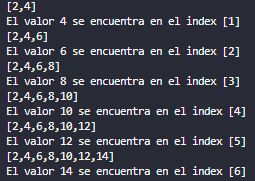
\includegraphics[width=1\linewidth]{images/busquedarecursiva.png}
  \\
  Figura 5. Ejecución algoritmo de búsqueda recursiva.
\end{minipage}\hfill
\begin{minipage}{.45\linewidth}
  \centering
  \begin{tabular}{|c|c|}
    \hline
    \textbf{Valor de $n$} & \textbf{\# de pasos} \\
    \hline
    2  & 13 \\
    3  & 13 \\
    4  & 13 \\
    5  & 18 \\
    6  & 18 \\
    7  & 18 \\
    8  & 18 \\
    9  & 18 \\
    10 & 18 \\
    11 & 18 \\
    12 & 18 \\
    13 & 18 \\
    14 & 23 \\
    15 & 23 \\
    \vdots & \vdots\\
    \hline
  \end{tabular}
  \\
  Tabla 6. Datos de algoritmo de búsqueda recursiva.
\end{minipage}

\medskip

Los datos de ejecución del algoritmo de búsqueda iterativa se muestran en la figura k. El algoritmo muestra un
crecimiento logaritmico base 3.
\begin{figure}[h]
  \begin{center}
    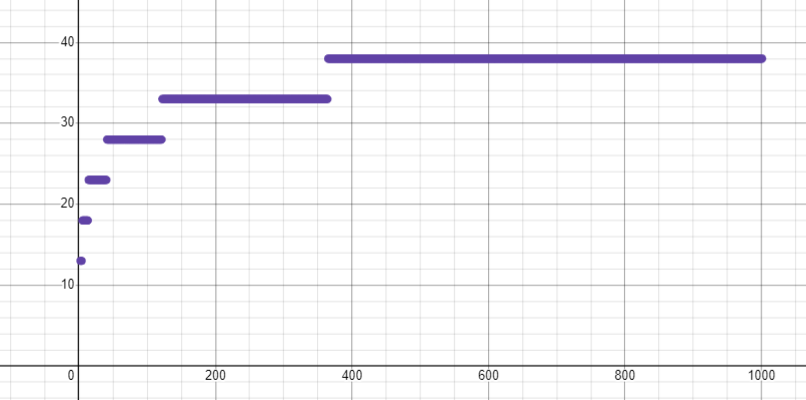
\includegraphics[width=0.7\linewidth]{images/busquedarecursivaworstcase.png}
    \\
    Figura k. Gráfica del comportamiento del algoritmo de búsqueda recursiva.
  \end{center}
\end{figure}
\newpage
En la figura 7 se muestra la función tal que $g(n)=8log_3(n)$ acota por arriba al algoritmo. El ajuste asíntotico es para cuando $n_0\geq 120$. En la figura 8 se muestra que $f(n)$ esta delimitado por $g(n)$ cuando $n\geq n_0$.

\begin{figure}[h]
  \begin{center}
    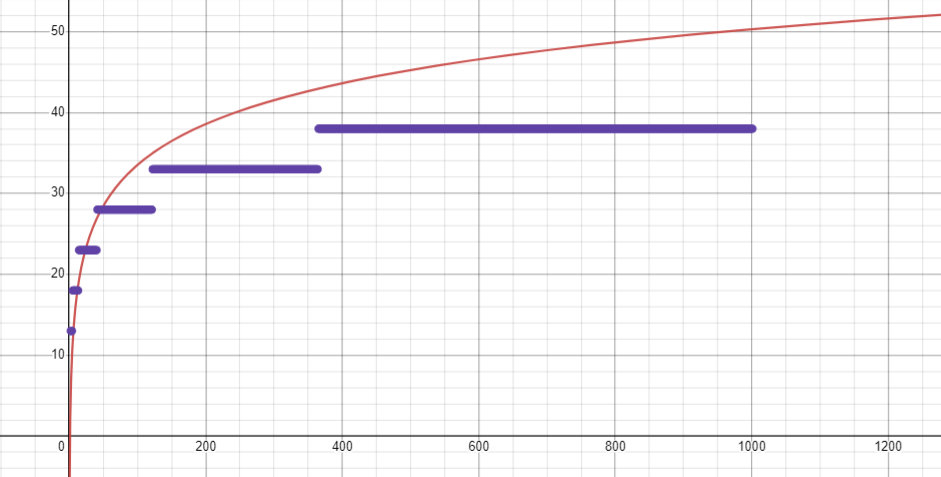
\includegraphics[width=0.7\linewidth]{images/busquedarecursivaworstcasegn.png}
    \\
    Figura 7. Gráfica con acotación para $f(n)$.
  \end{center}
\end{figure}
\begin{figure}[h]
  \begin{center}
    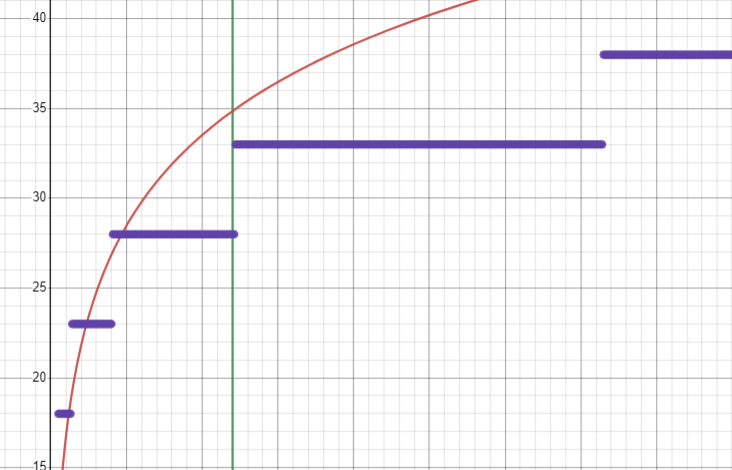
\includegraphics[width=0.5\linewidth]{images/busquedarecursivaworstcasegncota.png}
    \\
    Figura 8. Gráfica para valor $n_0$.
  \end{center}
\end{figure}


Por lo tanto, en el análisis a posteriori se muestra que el algoritmo es:
\begin{center}
  $\therefore T(n)\in O(log_3n)$
\end{center}

La comparación del algoritmo recursivo e iterativo tienen la misma complejidad temporal, como se desmuestra anteriormente, siendo ambos
big $O(log_3n)$, por lo que, para la búsqueda se puede implementar tanto de la forma recursiva o de la forma iterativa ya que tienen a misma eficiencia
en términos complejidad temporal. 

Sin embargo, es importante mencionar que el análisis de complejidad espacial se omite en los algoritmos que se presentan, ya que solo se desmuestra la complejidad temporal.

\newpage
\section{Conclusiones}

Un algoritmo se puede plantear de una forma recursiva en algunos casos o de forma iterativa, al final los dos algoritmos tienen la misma finalidad que es resolver un problema de una forma completa o parcial, lo importante es conocer cuál algoritmo es eficiente en complejidad temporal para un caso práctico, por lo que, es importante conocer las complejidades de las implementaciones de los algoritmos, ya sean recursivos o iterativos, por lo que, conociendo las complejidades se puede analizar cuál es eficiente para un caso práctico. Algunos algoritmos tienen la misma complejidad en su forma recursiva e iterativa, pero esto no siempre se cumple, ya que existen casos en los cuales el algoritmo recursivo es eficiente en comparación a su forma iterativa en complejidad temporal. Los algoritmos recursivos pueden ser complejos de calcular la complejidad temporal, ya que requieren de métodos de solución para las ecuaciones de recurrencia, entre los métodos están: la sustitución hacía atrás, método maestro, etc.

Por otra parte, es importante la complejidad espacial, ya que los algoritmos recursivos se tienen que tomar la complejidad espacial en cuenta, pero en esta práctica se omitió. 

\medskip

Conclusiones Catonga Tecla Daniel Isaí 1
\par
En esta práctica aprendí a analizar algoritmos recursivos y a compararlos con su forma iterativa, se conoció que algunos algoritmos recursivos tienen la misma complejidad que los iterativos, es decir que los dos son eficientes, aunque esto depende de la implementación del algoritmo, ya que un algoritmo puede tener la misma finalidad, pero por la implementación no tiene la misma complejidad, por lo que, siempre se tiene que buscar el eficiente en complejidad temporal. Por otra parte, el algoritmo de búsqueda fue interesante, ya que al dividir en tres partes nuestro arreglo ordenado, es menos eficiente que si solo lo vamos dividiendo a la mitad, y esto se demuestra solucionando las ecuaciones de recurrencia y obteniendo lo complejidad.

\medskip

Conclusiones Olguin Castillo Victor Manuel 2
\par
Texto ejemplo.

\newpage
\section{Bibliograf\'ia}

\printbibliography[title={ }]

\end{document}
